\section*{Глава 2. Аналитические и численные методы решения задач неизотермической фильтрации.}
\addcontentsline{toc}{section}{Глава 2. Аналитические и численные методы решения задач неизотермической фильтрации.}
\setcounter{section}{2}
\setcounter{subsection}{0}
\setcounter{equation}{0}

\subsection{Метод функций Грина}
	Метод функций Грина означает представление решения смешанной (краевой) задачи для дифференциального уравнения в частных производных в виде ряда по собственным функциям дифференциального оператора в опеределённой  области с определёнными граничными условиями \cite{vladimirov}.
	Это означает, что сам вид собственных функции дифференциального оператора зависит от формы области и граничных условий.
	
	Ниже будет рассмотрено применение метода к уравнению пьезопроводности, уравнению Пуассона в прямоугольной однородной области \cite{aziz_green}. Будет показана методика использования метода в задачах многофазной многокомпонентной фильтрации.

\subsubsection{Метод Фурье разделения переменных}
		Рассмотрим область $G \subset \mathbb{E}^3$ евклидового пространства, представляющую собой прямоугольный параллелепипед: $G = \{0 \leq x \leq s_x, 0 \leq y \leq s_y, 0 \leq z \leq s_z\}$, окружённую кусочно-гладкой границей $\Gamma = \Gamma_s \cup \Gamma_b \cup \Gamma_t$, где $\Gamma_t$ -- грань $z=s_z$, $\Gamma_b$ -- грань $z=0$, $\Gamma_s$ -- все остальные грани параллелепипеда.
	
	Рассмотрим уравнение пьезопроводности в области $G$:
\begin{equation}
	\label{piezo}
	\frac{\partial{p}}{\partial{t}} = \text{div}\left(\kappa\,\text{grad}\,p\right) + F\left(\boldsymbol{r}, t\right),
\end{equation}
	где $\kappa = \displaystyle\frac{k}{\mu m\beta}$ -- коэффициент пьезопроводности,
	$k$ -- проницаемость,
	$m$ -- пористость,
	$\beta$ -- полная сжимаемость,
	$F = \displaystyle\frac{Q(\boldsymbol{r},t )}{m\beta}$ -- функция источника, 
	$Q(\boldsymbol{r},t )$ -- объёмный расход флюида.
	Зададимся начальным условием:
\begin{align}
	\label{initial}
	p|_{t = 0} = p_0,
\end{align}		
	граничными условиями:
\begin{align}
	\label{boundary}
	p|_{\Gamma_s} = p_0, \quad \left.\frac{\partial{p}}{\partial{z}}\right|_{\Gamma_t, \Gamma_b} = 0,
\end{align}	
	что соответствует поддержанию постоянного давления $p_0$ на контуре и непротеканию через кровлю и подошву.
	
	Таким образом задача \eqref{piezo}, \eqref{initial}, \eqref{boundary} -- смешанная задача для неоднородного параболического уравнения с переменными коэффициентами.
	
	Применим метод Фурье для решения задачи \eqref{piezo}, \eqref{initial}, \eqref{boundary}, а именно будем искать её решение в виде:
\begin{equation}
	\label{sol}
	p(\boldsymbol{r},t) = \sum_{k=1}^\infty T_k(t)X_k(\boldsymbol{r}),
\end{equation}
	где $X_k$ -- ортонормальная система собственных функций дифференциального оператора $L = -\text{div}\left(\kappa\,\text{grad}\right)$.
		
	Получим вид функций $T_k$, умножим \eqref{piezo} на $X_k$ скалярно:
\begin{align}
	\label{st1}
	\int\limits_G \frac{\partial{p}}{\partial{t}} X_k d\boldsymbol{r} = \frac{d}{dt}\int\limits_G p X_k d\boldsymbol{r} =
	\frac{d}{dt}\left(p, X_k\right) = \nonumber\\
	=-\left(Lp, X_k\right) + \left(F, X_k\right) = -\lambda_k\left(p, X_k\right) + \left(F, X_k\right),
\end{align}
	где $\lambda_k$ -- собственные значения $L$, соответствующие собственным функциям $X_k$. Здесь использовался факт, что оператор $L$ -- эрмитов. Из \eqref{sol} имеем:
\begin{align}
	\label{state2}
	\left(p, X_k\right) = T_k.
\end{align}	
	Тогда из \ref{st1} получим уравнение на $T_k$:
\begin{align}
	\label{time_eq}
	T'_k = -\lambda_k T_k + \left(F, X_k\right), \\
	\left.T_k\right|_{t=0}=\left(p_0, X_k \right),
\end{align}
	решением которого будет:
\begin{align}
	\label{time_sol}
	T_k(t) &= \left(\left(p_0, X_k\right) + \left(F, X_k\right) \ast \right)e^{-\lambda_k t} =\\
	&= e^{-\lambda_k t}\int\limits_G p_0(\boldsymbol{r})X_k(\boldsymbol{r})d\boldsymbol{r}+
	\int\limits_0^t\int\limits_G F(\boldsymbol{r}', t') X_k(\boldsymbol{r}')d\boldsymbol{r}' e^{-\lambda_k (t-t')}dt',\nonumber
\end{align}
	где символом ''$\ast$'' обозначена свёртка. Вынося начальные условия в функцию источника $F$, решением \eqref{time_sol} будет, как известно, свёртка $F$ и фундаментального решения дифференциального оператора -- $e^{-\lambda_k t}$.

	Решение \eqref{sol} предстанет в виде:
\begin{align}
	\label{sol1}
	p\left(\boldsymbol{r}, t\right) &= \sum_{k=1}^\infty X_k(\boldsymbol{r}) \left(\left(p_0, X_k\right) + \left(F, X_k\right) \ast\right) e^{-\lambda_k t}
\end{align}
	В случае, если $p_0 = const$ то её можно вычесть и получить выражение при $p_0=0$. Меняя местами суммирование и интегрирование, получим:
\begin{align}
	\label{sol2}
	p\left(\boldsymbol{r}, t\right) &= \int\limits_G \int\limits_0^t F\left(\boldsymbol{r}', t\right) G(\boldsymbol{r},\boldsymbol{r}', t-t') dt' d\boldsymbol{r'},\\
	G(\boldsymbol{r},\boldsymbol{r}', t-t') &= \sum_{k=1}^\infty X_k(\boldsymbol{r}) X_k(\boldsymbol{r}') e^{-\lambda_k(t-t')},
\end{align}
	где $G(\boldsymbol{r}, \boldsymbol{r}', t-t')$ -- \textit{функция мнгновенного точечного источника} или \textit{функция Грина}.
	
	Систему собственных функций оператора $L$ выберем так, чтобы она удовлетворяла граничным условиям \eqref{boundary}:
\begin{equation}
	\label{eigenfuncs}
	\sqrt{\frac{8}{s_x s_y s_z}}\text{sin}\left(\frac{\pi n_x x}{s_x}\right)\text{sin}\left(\frac{\pi n_y y}{s_y}\right)\text{cos}\left(\frac{\pi n_z z}{s_z}\right)
\end{equation}
	Функция Грина $G$ примет вид:
\begin{align}
	\label{green}
	G(\boldsymbol{r},\boldsymbol{r}', t-t') &= \frac{8}{V}\sum_{n_x, n_y, n_z = 0}^\infty \chi_{n_x, n_y, n_z} e^{-\lambda_{n_x, n_y, n_z}(t-t')}\\
	 \chi_{n_x, n_y, n_z}(x, y, z, x', y', z') &= \text{sin}\left(\frac{\pi n_x x}{s_x}\right)\text{sin}\left(\frac{\pi n_y y}{s_y}\right)\text{cos}\left(\frac{\pi n_z z}{s_z}\right) \cdot \nonumber\\
	&\cdot\text{sin}\left(\frac{\pi n_x x'}{s_x}\right)\text{sin}\left(\frac{\pi n_y y'}{s_y}\right)\text{cos}\left(\frac{\pi n_z z'}{s_z}\right), \nonumber\\
	 \lambda_{n_x, n_y, n_z} &= \kappa \pi^2 \left(\frac{n_x^2}{s_x^2}+\frac{n_y^2}{s_y^2}+\frac{n_z^2}{s_z^2}\right),
\end{align}	
	где $V = s_x s_y s_z$ -- объём параллелепипеда.
	
	В стационарном случае будем иметь:
\begin{align}
	\label{sol_st}
	p\left(\boldsymbol{r}\right) &= \int\limits_G Q\left(\boldsymbol{r}'\right) G(\boldsymbol{r},\boldsymbol{r}') d\boldsymbol{r'} \\
	G(\boldsymbol{r}, \boldsymbol{r}') &= \frac{8k}{V\mu}\sum_{n_x, n_y, n_z = 0}^\infty \frac{\chi_{n_x, n_y, n_z}}{\lambda_{n_x, n_y, n_z}}\nonumber\\
	\lambda_{n_x, n_y, n_z} &= \pi^2\left(\frac{n_x^2}{s_x^2}+\frac{n_y^2}{s_y^2}+\frac{n_z^2}{s_z^2}\right)\nonumber
\end{align}

\subsubsection{Проблемы сходимости рядов}
	К сожалению ряды \eqref{sol2}, \eqref{sol_st} -- условно сходящиеся. Это означает, что их частичные суммы плохо сходятся и необходимо огромное количество итераций для получения результата с приемлемой точностью.

	Вопросы сходимости этих рядов и методы их суммирования рассмотрены в \cite{posv1}, \cite{posv2}.
	Там же предложен метод Эвальда для суммирования этих рядов.
	Метод впервые был предложен для суммирования подобных рядов в физике твёрдого тела.
	Опишем вкратце этот метод для стационарного случая.

	В выражении для функции Грина \eqref{sol_st} производится следующее преобразование:
\begin{equation}
	\label{transformation1}
	\frac{1}{\lambda_{n_x, n_y, n_z}} =
	\int\limits_{0}^{\xi_c}\exp(-\lambda_{n_x, n_y, n_z}\xi)d\xi+
	\int\limits_{\xi_c}^{\infty}\exp(-\lambda_{n_x, n_y, n_z}\xi)d\xi.
\end{equation}

	Плохо сходящийся ряд, который содержит первый интеграл, суммируется в пространстве Фурье с помощью формулы Пуассона, которая в данном случае позволит посчитать ряд:
\begin{multline}
	\label{statement}
	\frac{2}{s_x}\sum\limits_{n_x=0}^{\infty} \exp\left(-\frac{\pi^2 n_x^2 \xi}{s_x^2}\right)\sin\left(\frac{\pi n_x x}{s_x}\right)\sin\left(\frac{\pi n_x x'}{s_x}\right) =\\
	=\frac{1}{2\sqrt{\pi \xi}}\sum\limits_{i = -\infty}^{+\infty}\left[\exp\left(-\frac{(x-x'+2is_x)^2}{4\xi}\right)-\exp\left(-\frac{(x+x'+2is_x)^2}{4\xi}\right)\right],
\end{multline}
	который сходится по $i$ гораздо лучше.

	Ряд содержащий второй интеграл суммируется напрямую, его скорость сходимости достаточно хорошая.
	Таким образом можно посчитать плохо сходящиеся ряды вида \eqref{sol_st}, за приемлимое время.

\subsubsection{Случай многофазной многокомпонентной фильтрации}
	Метод может быть использован для расчёта многофазной многокомпонентной фильтрации, 
	необходимо лишь привести соответствующие уравнения к уравнению Пуассона (здесь, также для простоты, рассмотрим стационарный случай, обобщение на нестационарный случай \eqref{sol2} получается без труда).

	Это можно осуществить использую \textit{функцию Христиановича} (\textit{generalized pseudopressure function}) \cite{multiphase}.
	Запишем закон сохранения массы для каждой компоненты:
\begin{equation}
	\label{eq1}
	\text{div}\sum_{\alpha=1}^{k}\frac{k_\alpha\rho_\alpha l_{i\alpha}}{\mu_\alpha}\nabla p = Q_i, \quad \sum_{i = 1}^{n}l_{i\alpha} = 1, \quad i = \overline{1, n}, \quad \alpha = \overline{1, k},
\end{equation}
	где $i$ обозначает компоненту, $\alpha$ -- фазу,
	$l_{i\alpha}$ -- массовая доля $i$-ой компоненты в $\alpha$-ой фазе,
	$Q_i$ -- массовый источник.
	Суммируя \eqref{eq1} по всем компонентам, получим:
\begin{equation}
	\label{eq2}
	\text{div}\sum_{\alpha=1}^{k}\frac{k_\alpha\rho_\alpha }{\mu_\alpha}\nabla p = Q.
\end{equation}

	Введём функцию Христиановича для отдельной компоненты и для всего флюида в следующей форме:
\begin{equation}
	\label{eq3}
	H_i = \int\sum_{\alpha=1}^{k}\frac{k_\alpha\rho_\alpha l_{i\alpha}}{\mu_\alpha}dp + C, \quad
	H = \int\sum_{\alpha=1}^{k}\frac{k_\alpha\rho_\alpha }{\mu_\alpha}dp + C.
\end{equation}
	Тогда уравнения \eqref{eq1}, \eqref{eq2} могут быть записаны в виде:
\begin{equation}
	\label{eq4}
	\nabla^2 H_i = Q_i, \quad \nabla^2 H = Q,
\end{equation}
	т.е. в виде уравнения Пуассона.
	
	Однако необходимо ещё получить давление из преобразований \eqref{eq3}, которые являются функциями следующих неизвестных: $\{s_\alpha, l_{i\alpha}\}$, $s_{\alpha}$ -- насыщенности.
	Чтобы избавится от этих зависимостей введём понятие \textit{компонентного фактора} $\Gamma_i$:
\begin{equation}
	\label{eq5}
	\Gamma_i = \frac{\displaystyle\sum_{\alpha=1}^{k}\frac{k_\alpha\rho_\alpha l_{i\alpha}}{\mu_\alpha}}{\displaystyle\sum_{\alpha=1}^{k}\frac{k_\alpha\rho_\alpha}{\mu_\alpha}}, \quad i = \overline{1, n},
\end{equation}	
	который постоянен вдоль линий тока в стационарном случае:
\begin{equation}
	\label{eq6}
	\nabla\Gamma_i = 0, \quad i=\overline{1, n}.
\end{equation}

	В двухфазном случае (газожидкостная смесь) \eqref{eq6} может быть записано в виде:
\begin{equation}
	\label{eq7}
	 \frac{k_g\rho_g\mu_l}{k_l\rho_l\mu_g} = \frac{l_i - \Gamma_i}{\Gamma_i-g_i} = \dots = \frac{l_{n-2} - \Gamma_{n-2}}{\Gamma_{n-2}-g_{n-2}}, \quad  i = \overline{1, n},
\end{equation}
	где нижние индексы $\{l, g\}$ обозначают жидкую и газовую фазы соответственно,
	$l_i$, $g_i$ -- массовая доля $i$-ого компонента в жидкой и газовой фазах.
	В случае, когда мы знаем компонентный фактор $\Gamma_i$, мы можем решить \eqref{eq7} и определить $\{s_l, l_1, \cdots, l_{n-2}\}$ как функции давления $p$. Подставляя их в \eqref{eq3} получим забойное давление.


\subsection{Метод контурных интегралов}
	Как известно краевая задача для уравнения Пуассона может быть сведена к интегральному уравнению Фредгольма II-го рода. В определённых случаях в уравнении остаётся лишь интеграл по контуру, который при некоторых предположениях может быть посчитан аналитически. 
	
	Ниже будет представлен общий подход \textit{метода контурных интегралов} для решения уравнения Пуассона, а также пример расчёта забойного давления в скважине.
	
	Подробное применение метода, а также более серьезное рассмотрение \textit{метода граничных элементов} в применении к задачам фильтрации представлено в \cite{diss}.
	В статье \cite{main} предлагается новый подход для расчёта индекса скважины (well index) на основе метода контурных интегралов при полноценном гидродинамическом моделировании на неструктурированных сетка для скважин произвольной геометрии.
	
\subsubsection{Общий подход}
	Рассмотрим дифференциальное уравнение в виде:
\begin{align}
	\label{poisson}
	\mathcal{L}(p) = -\sigma,
\end{align}
	где $\mathcal{L}$ -- самосопряжённый дифференциальный оператор,
	$\sigma$ -- функция источника внутри области.
	Будем решать его в области $\Omega$, окружённой кусочно-гладкой границей $\Gamma = \Gamma_w \cup \Gamma_i$. 
	Рассмотрим дифференциальный оператор второго порядка вида:
\begin{align}
	\label{operator}
	\mathcal{L}(p) = \sum_{i,j=1}^{n}\frac{\partial^2(a_{ij}p)}{\partial x_i \partial x_j} + \sum_{i=1}^n \frac{\partial(b_i p)}{\partial x_i} + cp, 
\end{align}

	В \cite{math} показано, что для такого оператора $\mathcal{L}$ верна \textit{вторая формула Грина}, записанная в общей форме:
\begin{align}
	\label{formula}
	\int\limits_\Omega \left[u\mathcal{L}(v)-v\mathcal{L}(u)\right]d\omega = \int\limits_\Gamma \mathbb{A}\left[u\nabla v - v\nabla u\right] \vec{n}d\gamma,
\end{align}
	где $u, v$ -- произвольные достаточно гладкие функции,
	$\mathbb{A} = a_{ij}$.
	
	Введём функцию Грина пустого пространства - $G$, удовлетворяющую уравнению:
\begin{equation}
	\label{green}
	\mathcal{L}(G) + \delta(\mathbf{x}-\mathbf{x}') = 0,
\end{equation}
	где $\mathbf{x}'$ -- точечный источник, место где решение уходит в бесконечность.
	
	Тогда запишем \eqref{formula} для функций $p$, $G$:
\begin{equation}
	\label{form1}
	\int\limits_\Omega \left[p\mathcal{L}(G)-G\mathcal{L}(p)\right]d\omega = \int\limits_\Gamma \mathbb{A}\left[p\nabla G - G\nabla p\right] \cdot \mathbf{n}d\gamma.
\end{equation}
	
	Уточним оператор $\mathcal{L}$:
\begin{align}
	\label{operator1}
	\mathcal{L}(p) = \nabla(\mathbb{K}\nabla p).
\end{align}
	Из \eqref{form1} получим:
\begin{align}
	\label{form2}
	c(\mathbf{x}')p(\mathbf{x}') &= \int\limits_\Gamma \left[p(\mathbf{x})F_n(\mathbf{x}-\mathbf{x}')-q_n(\mathbf{x})G(\mathbf{x}-\mathbf{x}')\right]d\gamma + \int\limits_\Omega \sigma(\mathbf{x}) G(\mathbf{x}-\mathbf{x}') d\omega,\\
	F_n &= \mathbf{F} \cdot \mathbf{n} = -\mathbb{K}\nabla G \cdot \mathbf{n},\\
	q_n &= \mathbf{q} \cdot \mathbf{n} = -\mathbb{K}\nabla p \cdot \mathbf{n},
\end{align}	
	где $c(\mathbf{x'}) = \frac{\theta}{2\pi}$, где $\theta$ иммет смысл угла под которым видна область $\Omega$ внутри замыкания, и $\theta = 0$ вне замыкания:
\begin{equation}
	\label{cc}
	c(\mathbf{x}') =  
	\begin{cases}
    		1       & \quad \mathbf{x}' \in {\Omega} \backslash \Gamma, \\
    		\displaystyle\frac{\theta}{2\pi}       & \quad \mathbf{x}' \in \Gamma \\
		0  & \quad \mathbf{x}' \notin \Omega \cup \Gamma \\
	\end{cases}
\end{equation}

	В случае отсутствия объёмных источников(за исключением скважины) выражение \eqref{form2} упрощается и принимает вид:
\begin{align}
	\label{form3}
	c(\mathbf{x}')p(\mathbf{x}') &= \int\limits_\Gamma \left[p(\mathbf{x})F_n(\mathbf{x}-\mathbf{x}')-q_n(\mathbf{x})G(\mathbf{x}-\mathbf{x}')\right]d\gamma.
\end{align}

\subsubsection{Пример}

	Рассмотрим двумерный случай - квадратную область со скважиной в центре. На границе зададим постоянное давление. Распишем для начала $G$ и $F_n$ в 2D:
\begin{align}
	\label{form4}
	G(\mathbf{x}-\mathbf{x}') &= \frac{-\text{ln\,R}}{2\pi\sqrt{K_x K_y}}, \quad
	F_n(\mathbf{x}-\mathbf{x}') = \frac{(\mathbf{x}-\mathbf{x}') \cdot \mathbf{n}}{2\pi\sqrt{K_x K_y}R^2}, \\
	R &= \sqrt{\frac{(x-x')^2}{K_x} + \frac{(y-y')^2}{K_y}},
\end{align}
	где $R$ -- расстояние между точками $\mathbf{x}$ и $\mathbf{x}'$ с учётом анизотропии.
	
	Для простоты примем, что $K_x = K_y \equiv K$. Поставим точку $\mathbf{x}'$ в центр скважины, т.е вне области. Тогда выражение \eqref{form3} предстанет в виде:
\begin{align}
	\label{form5}
	0 &= I_w + I_i, \\
	I_w &= \int\limits_0^{2\pi r_w}\left(p_w\frac{-r_w}{2\pi K R^2} - q_w\frac{-\text{ln}\,R}{2\pi K}\right)d\gamma = 
	-p_w + q_w\frac{r_w \text{ln}({r_w^2}/{K})}{2K},\\
	I_i &= 8 \int\limits_0^{L/2}\left(p_i\frac{L/2}{2\pi K R^2} - q_i\frac{-\text{ln}\,R}{2\pi K}\right)d\gamma =
	p_i + q_i \frac{L\left(\text{ln}(L^2/(2K))+\pi/2 - 2\right)}{\pi K}.
\end{align}
	Принимая, что:
\begin{align}
	\label{form6}
	q_w = \frac{QB}{2\pi r_w h}, \quad q_i = -\frac{QB}{Lh},
\end{align}	
	получим выражение:
\begin{align}
	\label{form7}
	p_i - p_w = \frac{QB}{2\pi K h} \left(\pi - 4 + \text{ln}\frac{L^4}{4K \sqrt{K}r_w}\right).
\end{align}	
	
\subsection{Метод конечных объёмов}
	При моделировании флюидодинамики нефтяных пластов широкое распространение получил \textit{метод конечных объёмов} или \textit{finite volume method} (FVM). 

	В основе метода лежит, отличная от метода конечных разностей, техника представления расчётной сетки.
	Если в методе конечных разностей расчётная область представляется в виде конечного числа узлов (node), образующих сетку, то в FVM область предсталяется как множество расчётных ячеек (cell).
	Значения неизвестных величин в ячейках отождествляются с соответствующими значениями в их центрах.
	Эти значения, как мы увидим ниже, есть ни что иное как среднее по объёму всей ячеки.

	Особенностью метода является то, что он оперирует к интегральным законам сохранения искомых величин.
	Это несколько сокращает спектр его применения, однако делает его предпочтительным для применения к решению соответствующих законов.
	Численная схема, получающаяся в результате использования метода является \textit{консервативной} относительно соответствующего закона сохранения.

	В этой связи, метод получил широкое распространение при расчётах механики жидкости и газа, механики твёрдого тела. 
	Ниже будет изложен сам метод и его непосредственное использование для решения поставленных уравнений \eqref{eqns2}, \eqref{energy_last}.
	Подробное изложение основ метода и его приложений к решению гиперболических уравнений представлено в \cite{leveque}.
	Использование метода для задач фильтрации описано в \cite{kanevskaya}.
	Там же приведены конкретные численные схемы и варианты аппроксимации потоков, используемые при гидродинамическом моделировании фильтрации.

\subsubsection{Основа метода}
	Рассмотрим закон сохранения вектора величин $\boldsymbol{q}$ в следующей форме:
\begin{equation}
	\label{num_cons}
	\frac{\partial \boldsymbol{q}}{\partial t} + \nabla \cdot \mathbb{F} = 0,
\end{equation}
	где $\mathbb{F}$ -- матрица потоков соответствующих величин $\boldsymbol{q}$.
	Как можно видеть вид рассматриваемого уравнения \eqref{num_cons} полностью соотвествует виду закона сохранения массы \eqref{mass_law_e_div} в подходе Эйлера.

	Уравнению \eqref{num_cons} соответствует \textit{интегральная форма закона сохранения} величины $\boldsymbol{q}$:
\begin{equation}
	\label{num_cons_int}
	\frac{d}{dt}\int\limits_{\Omega}\boldsymbol{q}dV + \oint\limits_{\partial \Omega}\mathbb{F}\cdot \boldsymbol{n}\, dS = 0,
\end{equation}
	где $\Omega \in \mathbb{E}^3$ -- рассматриваемая область, $\partial \Omega$ -- её граница,
	$\boldsymbol{n}$ -- вектор единичной нормали к поверхности $\partial \Omega$.

	В дальнейшем будем использовать цилиндрическую систему координат, хотя все приведённые ниже выкладки можно легко обобщить на другие СК. Имеем:
\begin{equation}
	\label{num_cons_int}
	\mathbb{F} = \left(\boldsymbol{F}_r\,\boldsymbol{F}_{\varphi}\,\boldsymbol{F}_z\right),
\end{equation}
	где $\boldsymbol{F}_r$, $\boldsymbol{F}_{\varphi}$, $\boldsymbol{F}_z$ -- векторы потоков вдоль соответствующих направлений.

	Рассмотрим ячейку $\Omega_{ijk}$, индекс $i$ соответствует радиальной координате, $j$ -- аксиальной, $k$ -- вертикальной. В этом случае, интегрируя закон \eqref{num_cons_int} по времени, получим:
\begin{align}
	\label{num_law1}
	&\int\limits_{\Omega_{ijk}}\left(\boldsymbol{q}(r, \varphi, z, t^{n+1})-\boldsymbol{q}(r, \varphi, z, t^{n})\right)dV =\nonumber\\
	&=\int\limits_{t^n}^{t^{n+1}}\int\limits_{\partial\Omega_{i+\frac{1}{2}}}\boldsymbol{F}(r_{i+\frac{1}{2}}, \varphi, z, t)r_{i+\frac{1}{2}}d\varphi dzdt
	-\int\limits_{t^n}^{t^{n+1}}\int\limits_{\partial\Omega_{i-\frac{1}{2}}}\boldsymbol{F}(r_{i-\frac{1}{2}}, \varphi, z, t)r_{i-\frac{1}{2}}d\varphi dzdt+\nonumber\\
	&+\int\limits_{t^n}^{t^{n+1}}\int\limits_{\partial\Omega_{j+\frac{1}{2}}}\boldsymbol{F}(r, \varphi_{j+\frac{1}{2}}, z, t)drdzdt
	-\int\limits_{t^n}^{t^{n+1}}\int\limits_{\partial\Omega_{j-\frac{1}{2}}}\boldsymbol{F}(r, \varphi_{j-\frac{1}{2}}, z, t)drdzdt+\nonumber\\
	&+\int\limits_{t^n}^{t^{n+1}}\int\limits_{\partial\Omega_{k+\frac{1}{2}}}\boldsymbol{F}(r, \varphi, z_{k+\frac{1}{2}}, t)rdrd\varphi dt
	-\int\limits_{t^n}^{t^{n+1}}\int\limits_{\partial\Omega_{k-\frac{1}{2}}}\boldsymbol{F}(r, \varphi, z_{k-\frac{1}{2}}, t)rdrd\varphi dt,
\end{align}
	где индекс $n$ соответствует шагам по времени, 
	а различные индексированные $\partial\Omega$ обозначают поверхности ячейки $\Omega_{ijk}$ при соответствующей координате.

	Введём обозначения вида:
\begin{align}
	\label{num_terms2}
	S_{i+\frac{1}{2}}\boldsymbol{F}_r^{+} &= \frac{1}{\Delta t^n} \int\limits_{t^n}^{t^{n+1}}\int\limits_{\partial\Omega_{i+\frac{1}{2}}}\boldsymbol{F}(r_{i+\frac{1}{2}}, \varphi, z, t)r_{i+\frac{1}{2}}d\varphi dzdt,\\
	S_{i-\frac{1}{2}}\boldsymbol{F}_r^{-} &= \frac{1}{\Delta t^n} \int\limits_{t^n}^{t^{n+1}}\int\limits_{\partial\Omega_{i-\frac{1}{2}}}\boldsymbol{F}(r_{i-\frac{1}{2}}, \varphi, z, t)r_{i-\frac{1}{2}}d\varphi dzdt,\\
	\boldsymbol{q}_{ijk}^{n} &= \frac{1}{V_{ijk}}\int\limits_{\Omega_{ijk}}\boldsymbol{q}(r, \varphi, z, t^{n})dV.
\end{align}
	Сответственно можно видеть, что $\boldsymbol{q}_{ijk}^n$ предсталяет собой среднее значение величин $\boldsymbol{q}$ в ячейке $\Omega_{ijk}$ в момент времени $t^n$, 
	$S_{i+\frac{1}{2}}$ -- площадь поверхности $\partial\Omega_{i+\frac{1}{2}}$,
	$S_{i+\frac{1}{2}}\boldsymbol{F}_r^{+}$ -- средний поток через поверхность $\partial\Omega_{i+\frac{1}{2}}$ за время $\Delta t^n = t^{n+1}-t^n$.
	
	Подставляя принятые обозначения в \eqref{num_law1}, получим:
\begin{equation}
	\label{num_law2}
	\boldsymbol{q}_{ijk}^{n+1}-\boldsymbol{q}_{ijk}^{n} = \frac{\Delta t^n}{V_{ijk}}
	\left[
	S_{i+\frac{1}{2}}\boldsymbol{F}_r^{+}-S_{i-\frac{1}{2}}\boldsymbol{F}_r^{-}+
	S_{j+\frac{1}{2}}\boldsymbol{F}_\varphi^{+}-S_{j-\frac{1}{2}}\boldsymbol{F}_\varphi^{-}+
	S_{k+\frac{1}{2}}\boldsymbol{F}_z^{+}-S_{k-\frac{1}{2}}\boldsymbol{F}_z^{-}
	\right].
\end{equation}
	Удобнее записать \eqref{num_law2} в форме:
\begin{equation}
	\label{num_law3}
	\boldsymbol{q}_{ijk}^{n+1}-\boldsymbol{q}_{ijk}^{n} = \frac{\Delta t}{V_{ijk}}
	\sum\limits_{\beta}S_{ijk, \beta}\boldsymbol{F}_{ijk, \beta},
\end{equation}
	где индекс в сумме пробегает следующие значения:
	$\beta=\{i\pm 1jk, ij\pm 1k, ijk\pm 1\}$,
	$S_{ijk, \beta}$, $\boldsymbol{F}_{ijk, \beta}$ -- площадь поверхности и средний поток между ячейками $ijk$, $\beta$.

	Выражение \eqref{num_law3} предсталяет собой численную схему метода конечных объёмов для трёхмерной системы законов сохранения вида \eqref{num_cons}.
	Эта схема и будет в дальнейшем применена для решения рассматриваемых уравнений.

\subsubsection{Схема для законов сохранения массы при двухфазной двухкомпонентной фильтрации}
	Здесь и далее будем рассматривать \textit{двухточечную аппроскимацию потоков} или \textit{two-point flux approximation} (TFPA).
	Запишем численную схему для уравнений \eqref{eqns2} на основе \eqref{num_law3}:
\begin{align}
	\label{pres_scheme}
	H^{(1)\,n+1}_{ijk} &= \left(\frac{\phi(p)S}{B_l(p)}\right)_{ijk}^{n+1} - \left(\frac{\phi(p)S}{B_l(p)}\right)_{ijk}^{n} + 
	\frac{\Delta t^n}{V_{ijk}}\sum T_{ijk, \beta}\frac{p_{ijk}^{n+1}-p_{\beta}^{n+1}}{\Delta x_{ijk, \beta}}
	\left(\frac{k_{rl}(S)}{\mu_l B_l(p)}\right)_{s}^{n+1},\\
	H^{(2)\,n+1}_{ijk} &= \left(\frac{\phi(p)(1-S)}{B_g(p)}+\frac{\phi(p)SRs(p)}{B_l(p)}\right)_{ijk}^{n+1} - \left(\frac{\phi(p)		(1-S)}{B_g(p)}+\frac{\phi(p)SRs(p)}{B_l(p)}\right)_{ijk}^{n} +\nonumber\\
	&+\frac{\Delta t^n}{V_{ijk}}\sum T_{ijk, \beta}\frac{p_{ijk}^{n+1}-p_{\beta}^{n+1}}{\Delta x_{ijk, \beta}}
	\left(\frac{k_{rg}(S)}{\mu_g B_g(p)}+\frac{k_{rl}(S)Rs(p)}{\mu_l B_l(p)}\right)_{s}^{n+1},
\end{align}
	где $\Delta x_{ijk, \beta}$ -- расстояние между центрами ячеек $ijk$ и $\beta$.
	Межблочные проводимости $T_{ijk, \beta}$ апроксимуруются как среднее гармоническое \cite{kanevskaya}:
\begin{equation}	
	\label{cond_appr}
	T_{ijk, \beta} = \frac{k_{ijk} k_{\beta}S_{ijk, \beta}}{k_{ijk} \Delta x_{\beta} + k_{\beta}\Delta x_{ijk}}
	(\Delta x_{ijk} + \Delta x_{\beta}),
\end{equation}
	где $\Delta x_{ijk}$ -- размер ячейки в соответствующем направлении (направление задаётся расположением соседа $\beta$).

	ОФП представляют собой сильные нелинейности (как зависимости насыщенности $S$), для которых хорошо себя зарекомендовала аппроксимация \textit{вверх по потоку} \cite{kanevskaya}:
\begin{equation}	
	\label{cond_appr1}
	s = 
	\begin{cases}
		ijk, &\quad p_{ijk}^n \geq p_{\beta}^n,\\
		\beta, &\quad p_{ijk}^n < p_{\beta}^n.
	\end{cases}
\end{equation}

	Затем схема \eqref{pres_scheme} линеаризуется по Ньютону.
	Пусть $\boldsymbol{H}_{ijk}^{n+1} = (H^{(1)\,n+1}_{ijk}, H^{(2)\,n+1}_{ijk})$ -- сеточная вектор-функция из двух компонент, $\boldsymbol{H}_{ijk}^{n+1} = \boldsymbol{H}(W^{n+1})$, где $W^{n+1} = \{p_{ijk}^{n+1}, S_{ijk}^{n+1}, p_{\beta}^{n+1}, S_{\beta}^{n+1}\}$.
	Напомним, что $\beta=\{i\pm 1jk, ij\pm 1k, ijk\pm 1\}$.
	Тогда запишем разложение в виде:
\begin{multline}
	\label{newton}
	\left.\frac{\partial \boldsymbol{H}_{ijk}^{l+1}}{\partial p_{ijk}^{l+1}}\right|_{W^{l}}\delta p_{ijk}^{l+1} + 
	\sum\limits_{\beta}\left.\frac{\partial \boldsymbol{H}_{ijk}^{l+1}}{\partial p_{\beta}^{l+1}}\right|_{W^{l}}\delta p_{\beta}^{l+1} + \\
	+\left.\frac{\partial \boldsymbol{H}_{ijk}^{l+1}}{\partial S_{ijk}^{l+1}}\right|_{W^{l}}\delta S_{ijk}^{l+1} + 
	\sum\limits_{\beta}\left.\frac{\partial \boldsymbol{H}_{ijk}^{l+1}}{\partial S_{\beta}^{l+1}}\right|_{W^{l}}\delta S_{\beta}^{l+1} = -\boldsymbol{H}_{ijk}^l,
\end{multline}
	где $l$ -- индекс итераций,
	$\delta p^{l+1} = p^{l+1}-p^{l}$, $\delta S^{l+1} = S^{l+1}-S^{l}$.

	Подобная схема записывается для каждой внутренней ячейки, затем замыкается подобными выражениями для граничных ячеек (будет обсуждено ниже), и, наконец, составляется СЛАУ относительно всех $\{\delta p_{ijk}^{l+1}, \delta S_{ijk}^{l+1}\}$. Данная система решается итерационно до достижения определённой дочности, потом проводится расчёт температуры, затем расчитывается следующий шаг по времени.

\subsubsection{Схема для уравнения баланса энергии}
	Для расчёта уравнения баланса энергии \eqref{energy_last} была использована комбинированная, полностью неявная, схема метода конечных объёмов и схема Кранка-Николсона \cite{petrov} для конвективных членов.
	Полученная итоговая численная схема имеет вид:
\begin{multline}
	\label{energy_scheme}
	H_{ijk}^{(3)\,n+1} = c_{t\, ijk}^{n+1}\left(\theta_{ijk}^{n+1}-\theta_{ijk}^{n}\right) + \\
	+\Delta t^n\sum\limits_{\beta}\left(a_{ijk, \beta}^{n+1}+\frac{\left(\tilde{\lambda}S\right)_{ijk, \beta}^{n+1}}{V_{ijk}}\right)
	\frac{\theta_{ijk}^{n+1}-\theta_{\beta}^{n+1}}{\Delta x_{ijk, \beta}}-\Delta t^{n} f_{ijk}^{n+1},
\end{multline}
\begin{align}
	\label{energy_scheme_terms}
	f_{ijk}^{n+1} &= \widetilde{c\eta}_{ijk}^{n+1}\frac{p_{ijk}^{n+1}-p_{ijk}^{n}}{\Delta t^{n}}-q_{ijk}^{n+1}L - 
	\sum\limits_{\beta}b_{ijk, \beta}^{n+1}\frac{p_{ijk}^{n+1}-p_{\beta}^{n+1}}{\Delta x_{ijk, \beta}},\nonumber\\
	q_{ijk}^{n+1} &= \frac{\left(\phi S \rho_l\right)_{ijk}^{n+1}-\left(\phi S \rho_l\right)_{ijk}^{n}}{\Delta t^{n+1}}+
	\sum\limits_{\beta}\frac{p_{ijk}^{n+1}-p_{\beta}^{n+1}}{\Delta x_{ijk, \beta}}T_{ijk, \beta}\left(\frac{k_{rl}}{\mu_l B_l}\right)_s,\nonumber\\
	a_{ijk, \beta}^{n+1}&=\text{max}\left(0, \text{sign}(x_{ijk}-x_{\beta})\widetilde{c v_x}_{ijk, \beta}\right),\nonumber\\
	b_{ijk, \beta}^{n+1}&=\text{max}\left(0, \text{sign}(x_{ijk}-x_{\beta})\widetilde{c \varepsilon v_x}_{ijk, \beta}\right),
\end{align}
	где $q_{ijk}^{n+1}$ -- интенсивность фазывых переходов,
	$T_{ijk, \beta}$ определяется выражением \eqref{cond_appr},
	величины $\widetilde{c v_x}_{ijk, \beta}$, $\widetilde{c \varepsilon v_x}_{ijk, \beta}$ аппроксимируются как средневзвешенные значения между ячейками $ijk$ и $\beta$.

	Поскольку уравнение \eqref{energy_last} -- линейное, решение по схеме \eqref{energy_scheme} находится за одну итерацию.

\subsubsection{Численное решение СЛАУ}

	В написанном расчётном модуле использовалось несколько вариантов солверов СЛАУ.

	При решении одно- и двумерных задач, линейная система сводилась к блочно-диагональному виду и решалась прогонкой.
	Для схемы \eqref{newton} блок имел размер $2\times2$ в одномерном случае, и $2n_z\times2n_z$ в двумерном, где $n_z$ -- размер сетки по оси $z$. Для схемы \eqref{energy_scheme} $1\times1$ в одномерном, $n_z\times n_z$ -- в двумерном.
	
	Безусловым преимуществом прогонки является скорость вычислений. Однако для подробных двумерных сеток это преимущество нивелируется. Уже при $n_z \sim 10$ скорость расчёта блочно-диагональной прогонки сравнима со скоростью расчёта итерационными методами.

	Интерационные методы применялись для решения двумерных и трёхмерных задач.
	Среди методов использовались методы крыловского подпространства -- GMRES, BiCGStab.
	Среди предобуславливателей -- ILU(0), ILU(1), ILU(2), ILUT(t, n).

	Несмотря на широкое использование обычной неполной факторизации (ILU) в некоторых случаях, с большими градиентами краевых условий (во времени), солвер не мог достичь заданной точности, и, как результат решение расходилось. Повышение порядка ILU факторизации не приносила успеха.
	В этом отношении предобуславливатель ILUT является более подходящим вариантом, который можно регулировать в зависимости от изменения условий.

	У солверов наблюдались характерные особенноти.
	Сходимость GMRES ухудшалась во времени при постоянном однотипном предобуславливании.
	BiCGStab расходился при больших возмущениях на границах.

	В качестве предобуславливателей и солверов использовалась сторонняя библиотека ''Paralution'', распространяющаяся по лицензии GPLv2. Исользовалась параллельная реализация библиотеки (OpenMP), т.е. расчёт производился в несколько потоков (до 12) на этапе решения СЛАУ.	

\subsubsection{Расчёт граничных ячеек и обсуждение граничных условий}
	Для расчёта границ в методе вводились так называемые фиктивные ячейки (ghost cell) нулевого размера вдоль оси, ортогональной границе. С помощью этих ячеек составлялась разностная схема для граничных условий \eqref{well_cond4}, \eqref{well_cond1}, \eqref{well_cond2}, \eqref{well_cond3} и \eqref{energy_contour3}, \eqref{energy_contour}.
	
	Для системы \eqref{eqns2} схемы для граничных условий также были подвергнуты линеаризации по Ньютону и, затем, итерационному решению в полной замкнутой СЛАУ.
	Поскольку система \eqref{eqns2} первого порядка по нефтенасыщенности $S$, для неё были поставлены условия лишь на одной границе вдоль каждой оси:
\begin{equation}
	\label{sat_bounds}
	\left.S\right|_{r=r_e} = S_0, \quad \left.\frac{\partial S}{\partial z}\right|_{z = 0} = 0,
\end{equation}
	где $S_0$ -- начальная нефтенасыщенность. Тогда как на другой границе значения нефтенасыщщености было линейно интерполировано.
	
	Аналогичная процедура применялась и для температуры на перфорированной поверхности скважины,  псокольку постановка граничного условия для подобной задачи представляет особые трудности.


\subsection{Распределение дебита вдоль ствола скважины}
	При расчёте с граничным условием \eqref{well_cond3} (контроль по дебиту) известен лишь суммарный дебит, а его распределение вдоль ствола подлежит определению.
	
	В основе используемого в данной работе метода распределния дебита лежит \textit{модель ствола скажины бесконечной проводимости}. 
	Это означает, что дебит распределяется так, чтобы давление во всех граничных перфорированных ячеек было едино.	
	Данная модель также распространяется и на вторичное вскрытие (каналы).

	Рассмотрим функционал $H = H(q_1, q_2, \cdots, q_K)$:
\begin{equation}
	\label{pres_functional}
	H = \frac{1}{2}\sum\limits_{k=1}^{K-1}\left(p_{k+1}-p_k\right)^2,
\end{equation}
	где суммирование проходит по всем перфориванным ячейкам.
	
	Неоходимо найти условный минимум функционала $\eqref{pres_functional}$ при условии:
\begin{equation}
	\label{functional_cond}
	\sum\limits_{k=0}^{K} q_k = Q.
\end{equation}
	
	Условие \eqref{functional_cond} эквивалентно сокращению колва аргументов $q_k$ на один.

	Линеаризуем давление:
\begin{equation}
	\label{press_linear}
	p_k = p_k^0 + \sum\limits_{i=1}^{K-1}\frac{\partial p_k}{\partial q_i}\Delta q_i,
\end{equation}
	и подставим его в \eqref{pres_functional}.

	Потребуем равенства всех частных производных $H$ по $\{q_1, \cdots, q_{K-1}\}$ нулю (необходимое условие локального экстремума).	
	Получим систему линейных уравнений относительно $\{q_1, \cdots, q_{K-1}\}$:
\begin{equation}
	\label{distr_system}
	\sum\limits_{i, k = 1}^{K-1}\left(\frac{\partial p_{k+1}}{\partial q_i} - \frac{\partial p_k}{\partial q_i}\right)
	\left(\frac{\partial p_{k+1}}{\partial q_j} - \frac{\partial p_k}{\partial q_j}\right)\Delta q_i = 
	-\sum\limits_{k=1}^{K-1}\left(p_{k+1}^0 - p_k^0\right)\left(\frac{\partial p_{k+1}}{\partial q_j} - \frac{\partial p_{k}}{\partial q_j}\right).
\end{equation}

	Последовательность нахождения распределения такова: 
\begin{enumerate}
	\label{rate_order}
	\item{Задаётся равномерное распределение дебитов $\{q_1, \cdots, q_{K}\}$.}
	\item{Производится решение задачи.}
	\item{В случае, если функционал \eqref{pres_functional} больше некоторого наперёд заданного значения производится его минимизация итерационно, пока не будет достигнута определённая точность.}
	\item{Производится переход к следующему временному слою. Перераспределение дебита будет производится если функционал \eqref{pres_functional} значительно возрастёт.}
\end{enumerate}

	Таким образом \eqref{distr_system} решается на каждом шаге по времени, когда \eqref{pres_functional} не удовлетворяет наперёд заданной точности.
	При этом для однофазной нефти задача распределения дебита (минимизация функционала) решается за одну итерацию, т.к. система линейна.
	В двухфазной постановке распределение дебита производится итерационно, поверх итераций численной схемы.

	На Рис. \ref{pic:part_pen1} представлена некоторая постановка скважины с неполным вскрытием и посчитанное установившееся распределение дебита отнесённое к равномерному.
\begin{figure}[H]

	\begin{subfigure}[b]{0.5\textwidth}
	\centering
	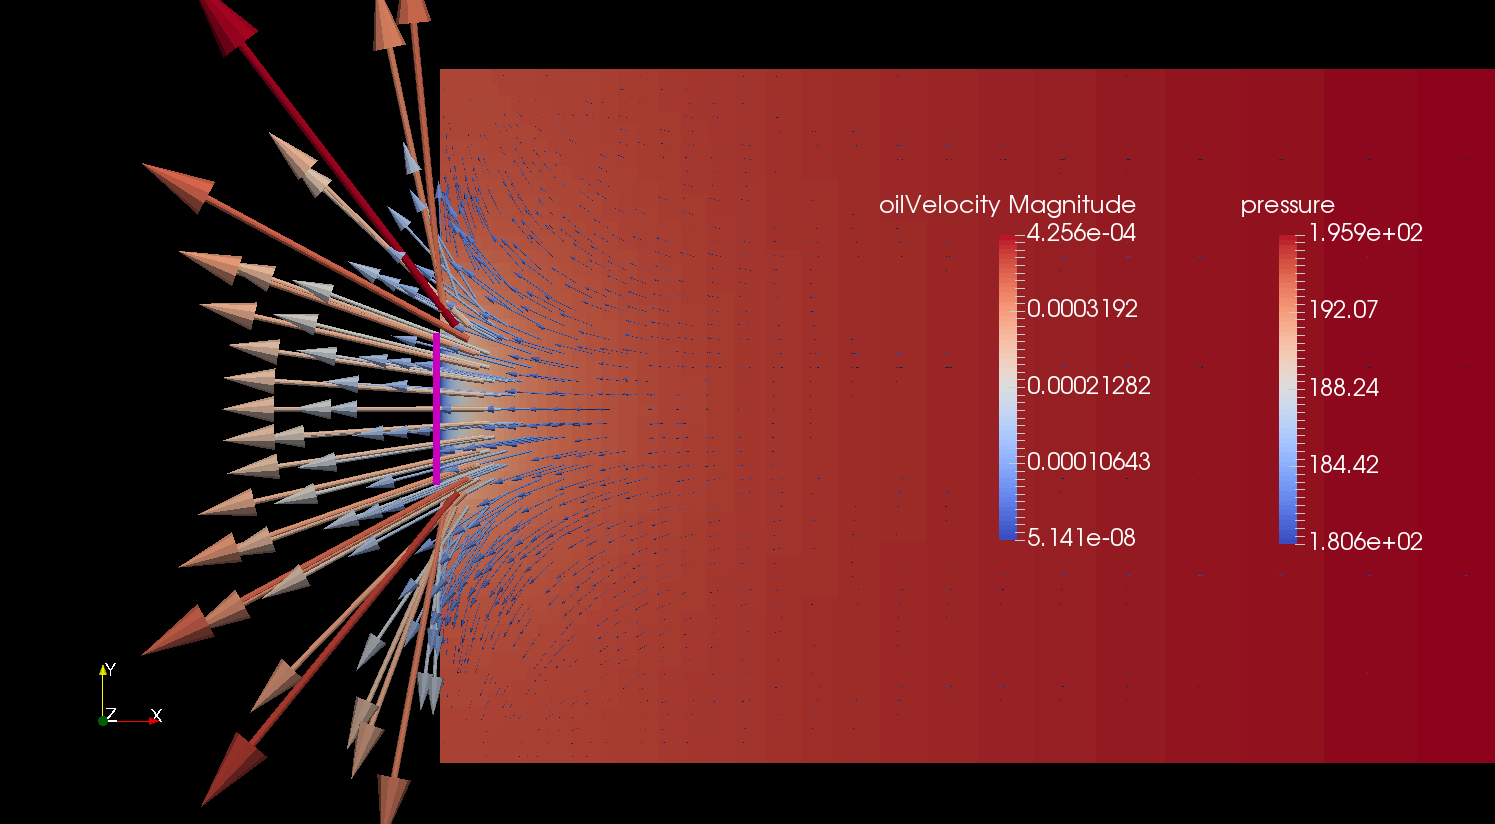
\includegraphics[width=1\textwidth]{pic/part_penetrating1.png}
	\caption{Постановка задачи с выделенной перфорированной областью}
	\label{pic:part_problem1}
	\end{subfigure}
~
	\begin{subfigure}[b]{0.5\textwidth}
		\centering
		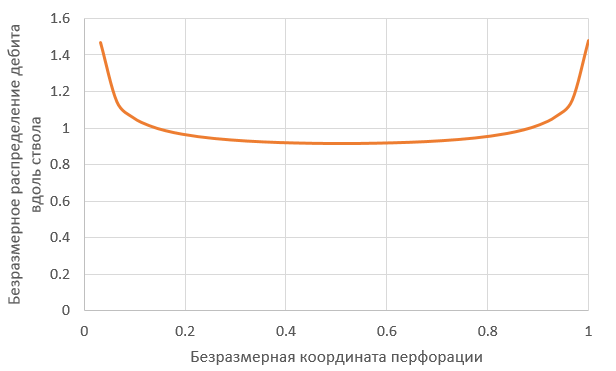
\includegraphics[width=1\textwidth]{pic/rate_distr1.png}
		\caption{Распределение дебита вдоль ствола}
		\label{pic:rate_distr1}
	\end{subfigure}
	\caption{Распределение дебита для скважины, частично вскрывающей пласт.}
	\label{pic:part_pen1}
\end{figure}
